\documentclass{beamer}
%
% Choose how your presentation looks.
%
% For more themes, color themes and font themes, see:
% http://deic.uab.es/~iblanes/beamer_gallery/index_by_theme.html
%
\mode<presentation>
{
  \usetheme{default}      % or try Darmstadt, Madrid, Warsaw, ...
  \usecolortheme{beaver} % or try albatross, beaver, crane, ...
  \usefonttheme{default}  % or try serif, structurebold, ...
  \setbeamertemplate{navigation symbols}{}
  \setbeamertemplate{caption}[numbered]
} 

\usepackage[english]{babel}
\usepackage[utf8x]{inputenc}
\usepackage{hyperref}
\hypersetup{
    colorlinks=true,
    linkcolor=blue,
    filecolor=magenta,      
    urlcolor=blue,
}

\title[Mapping]{Mapping}
\author{Andrés Pérez}
\institute{Digital Lutherie\\Master en Música para Experiencias del Entretenimiento\\ENTI-UB}
\date{2018/2019}

\newcommand\blfootnote[1]{%
  \begingroup
  \renewcommand\thefootnote{}\footnote{#1}%
  \addtocounter{footnote}{-1}%
  \endgroup
}

\AtBeginSection[]
{
\begin{frame}{Outline}
    \tableofcontents[currentsection,currentsubsection] 
\end{frame}
}

\begin{document}

\begin{frame}
  \titlepage
\end{frame}



\begin{frame}{Outline}
 \tableofcontents
\end{frame}

\begin{frame}{Mapping}
    \begin{figure}[h]
        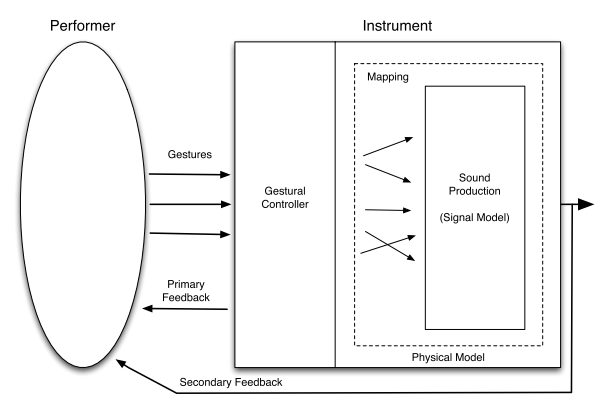
\includegraphics[width=0.9\textwidth]{instrument_scheme.png}\blfootnote{Wanderley, M. M. (2001). Performer-Instrument Interaction: Applications to Gestural Control of Sound Synthesis. PhD thesis, University Paris 6.}
    \end{figure}
\end{frame}


%%%%%%%%%%%%%%%%%%%%%%%%%%%%%%%%%%%%%%%%%%%%%%%%%%
\section{Definition}

\begin{frame}{Definition}
    \textit{"In an acoustic instrument, the playing interface is inherently bound up with the sound source. [...] Since they are inseparable, the connections between the two are complex, subtle and determined by physical laws. With electronic and computer instruments, the situation is dramatically different. [...] This means that the relationship between them has to be defined. The art of connecting these two, traditionally inseparable, components of a real-time musical system (an art known as \textbf{mapping}) is not trivial."}\footnote{Hunt, A., Wanderley, M. M., West, S. S., \& Paradis, M. (2002). The importance of parameter mapping in electronic instrument design. Proceedings of the 2002 Conference on New Instruments for Musical Expression (NIME-02).}
\end{frame}

\begin{frame}{Definition}
    \begin{figure}[h]
        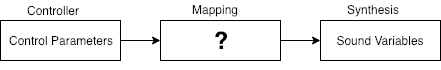
\includegraphics[width=\textwidth]{mapping.png}
    \end{figure}
\end{frame}

\begin{frame}{Definition}
    \begin{figure}[h]
        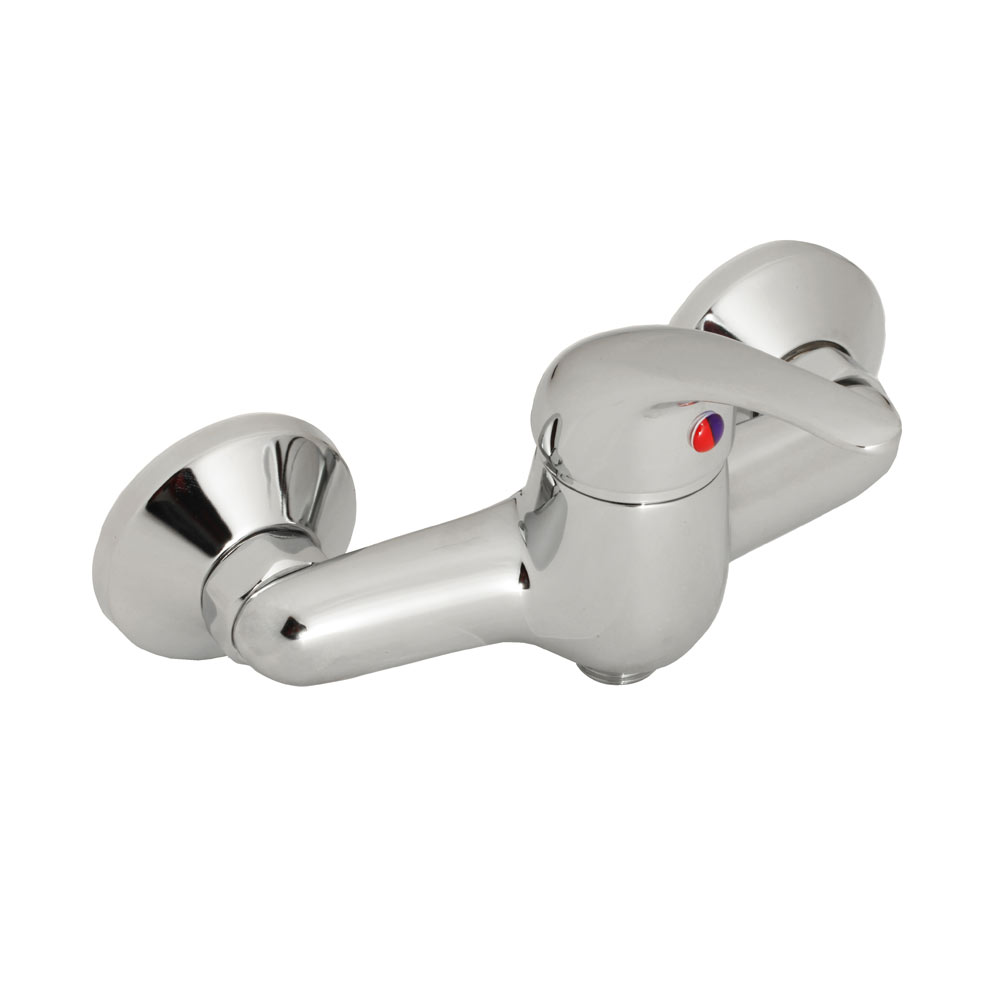
\includegraphics[width=0.7\textwidth]{grifo1.jpg}
    \end{figure}
\end{frame}

\begin{frame}{Definition}
    \begin{figure}[h]
        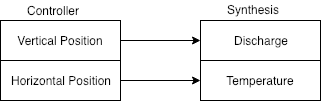
\includegraphics[width=0.7\textwidth]{grifo1_scheme.png}
    \end{figure}
\end{frame}

\begin{frame}{Definition}
    \begin{figure}[h]
        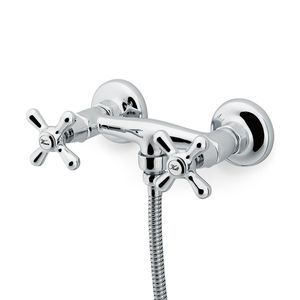
\includegraphics[width=0.7\textwidth]{grifo2.jpg}
    \end{figure}
\end{frame}

\begin{frame}{Definition}
    \begin{figure}[h]
        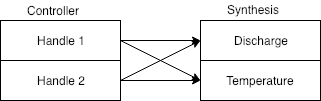
\includegraphics[width=0.7\textwidth]{grifo2_scheme.png}
    \end{figure}
\end{frame}

\begin{frame}{Definition}
    Which one is better?
\end{frame}

\begin{frame}{Definition}
    \begin{figure}[h]
        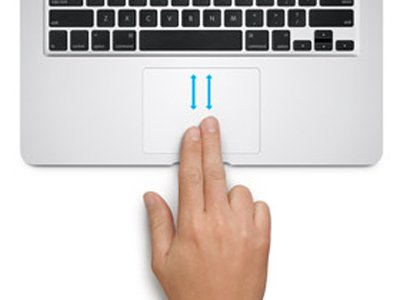
\includegraphics[width=0.8\textwidth]{scroll.jpg}
    \end{figure}
\end{frame}

\begin{frame}{Definition}
    Reverse scrolling vs. natural scrolling
        \begin{figure}[h]
        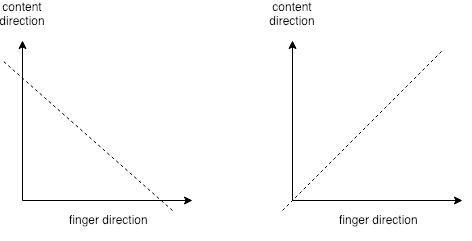
\includegraphics[width=0.8\textwidth]{scrolling_mapping.png}
    \end{figure}
\end{frame}

\begin{frame}{Definition}
    Which one is better?
\end{frame}

%%%%%%%%%%%%%%%%%%%%%%%%%%%%%%%%%%%%%%%%%%%%%%%%%%
\section{Taxonomy}

\begin{frame}{Taxonomy}
    \textbf{Mapping types}\\
    \vspace{5mm}
    \begin{itemize}
        \item One-to-one
        \begin{itemize}
            \item Each input parameter controls one sound variable.
            \item The most simple approach...
            \item Example: Theremin
         \end{itemize}
    \end{itemize}
\end{frame}

\begin{frame}{Taxonomy}
    \textbf{Mapping types}\\
    \vspace{5mm}
    \begin{itemize}
        \item One-to-one
        \begin{itemize}
            \item Each input parameter controls one sound variable.
            \item The most simple approach...
            \item Example: Theremin
         \end{itemize}
    \end{itemize}
    \begin{figure}[h]
        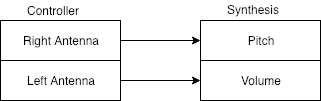
\includegraphics[width=0.7\textwidth]{theremin_mapping.png}
    \end{figure}
\end{frame}

\begin{frame}{Taxonomy}
    \textbf{Mapping types}\\
    \vspace{5mm}
    \begin{itemize}
        \item Many-to-one (converegent)
        \begin{itemize}
            \item Multiple input parameters control the same only sound variable.
            \item Example: Violin (\textit{"Where is the volume control?")}\footnote{Hunt, A. (2000). Mapping Strategies for Musical Performance.}
         \end{itemize}
    \end{itemize}
\end{frame}

\begin{frame}{Taxonomy}
    \textbf{Mapping types}\\
    \vspace{5mm}
    \begin{itemize}
        \item Many-to-one (converegent)
        \begin{itemize}
            \item Multiple input parameters control the same only sound variable.
            \item Example: Violin (\textit{"Where is the volume control?")}\footnote{Hunt, A. (2000). Mapping Strategies for Musical Performance.}
         \end{itemize}
    \end{itemize}
    \begin{figure}[h]
        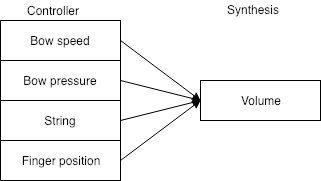
\includegraphics[width=0.5\textwidth]{violin_mapping1.png}
    \end{figure}
\end{frame}

\begin{frame}{Taxonomy}
    \textbf{Mapping types}\\
    \vspace{5mm}
    \begin{itemize}
        \item One-to-many (divergent)
        \begin{itemize}
            \item One input parameter controls many sound variables.
            \item Example: Violin (\textit{"Which sonic parameter does the bow control?")}\footnote{Hunt, A. (2000). Mapping Strategies for Musical Performance.}
         \end{itemize}
    \end{itemize}
\end{frame}

\begin{frame}{Taxonomy}
    \textbf{Mapping types}\\
    \vspace{5mm}
    \begin{itemize}
        \item One-to-many (divergent)
        \begin{itemize}
            \item One input parameter controls many sound variables.
            \item Example: Violin (\textit{"Which sonic parameter does the bow control?")}\footnote{Hunt, A. (2000). Mapping Strategies for Musical Performance.}
         \end{itemize}
    \end{itemize}
    \begin{figure}[h]
        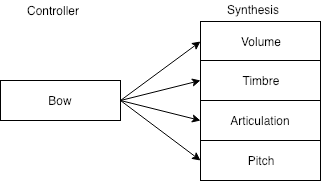
\includegraphics[width=0.5\textwidth]{violin_mapping2.png}
    \end{figure}
\end{frame}

\begin{frame}{Taxonomy}
    Acoustic instruments present multiple simultaneous convergent/divergent mappings...
\end{frame}

\begin{frame}{Taxonomy}
    Rovan's clarinet experiment\footnote{Hunt, A., Wanderley, M. M., West, S. S., \& Paradis, M. (2002). The importance of parameter mapping in electronic instrument design. Proceedings of the 2002 Conference on New Instruments for Musical Expression (NIME-02).}
        \begin{figure}[h]
        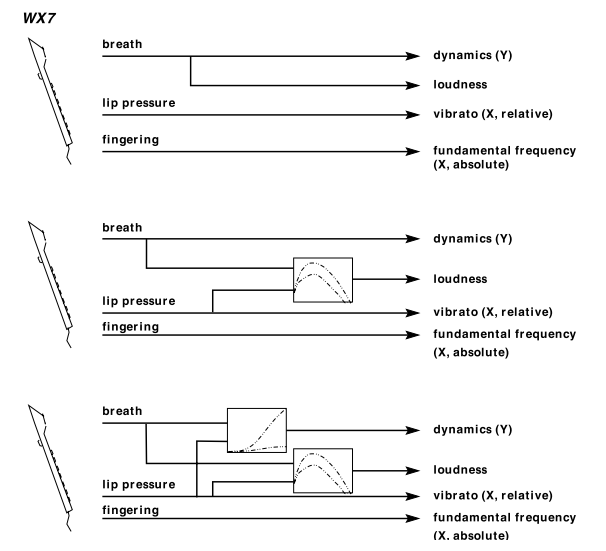
\includegraphics[width=0.6\textwidth]{clarinet_mapping.png}
    \end{figure}
\end{frame}

\begin{frame}{Taxonomy}
    Which one is better?
\end{frame}

% TODO: PONER EN LA PARTE DE EVALUATION
% \begin{frame}{Taxonomy}
%     Hunt's experiment\\
%     \vspace{5mm}
%     \textit{"Results indicated that wind instrument performers tended to stick with complex cross-coupled mappings similar to the single reed behaviour (the third mapping strategy used), whereas beginners initially preferred simpler mappings (easier to play and produce stable sounds)."}
% \end{frame}

\begin{frame}{Taxonomy}
    Hunt's Observation\footnote{Hunt, A., Wanderley, M. M., West, S. S., \& Paradis, M. (2002). The importance of parameter mapping in electronic instrument design. Proceedings of the 2002 Conference on New Instruments for Musical Expression (NIME-02).}
    \begin{figure}[h]
        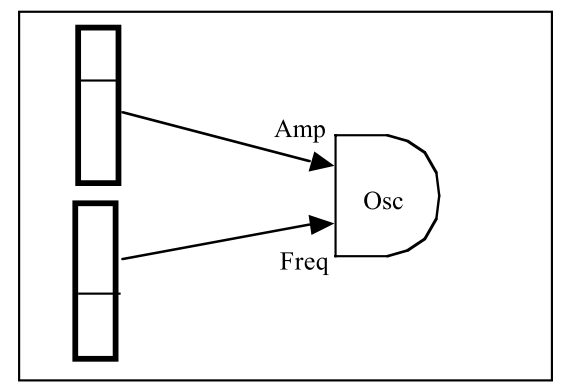
\includegraphics[width=0.5\textwidth]{hunt_simple.png}
        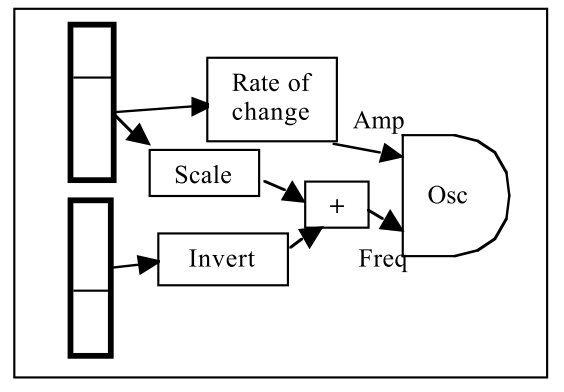
\includegraphics[width=0.5\textwidth]{hunt_complex.png}
    \end{figure}
\end{frame}

\begin{frame}{Taxonomy}
    Which one is better?
\end{frame}

%%%%%%%%%%%%%%%%%%%%%%%%%%%%%%%%%%%%%%%%%%%%%%%%%%

\section{Design Considerations}

\begin{frame}{Design Considerations}
    What about alternate controllers?
\end{frame}

\begin{frame}{Design Considerations}
    \begin{itemize}
        \item Metaphors
        \item Multi-level mappings
        \item Machine Learning
    \end{itemize}
\end{frame}

\subsection{Metaphors}
\begin{frame}{Design Considerations - Metaphors}
    General tendency to map gestures with parameters in a idiosyncratic way.
\end{frame}

\begin{frame}{Design Considerations - Metaphors}
    \textit{"In many real-time devices (for example a violin, a bicycle, a clarinet or a drum-kit) the human operator has to inject energy or ‘excite’ the system before it will operate, and must continue to supply energy to keep it going."}\footnote{Hunt, A. (2000). Mapping Strategies for Musical Performance.}
\end{frame}

\begin{frame}{Design Considerations - Metaphors}
    \textit{"[...] a wiring mistake by the student meant that the 'volume' antenna only worked when your hand was moving. [..] It was unexpectedly exciting to play. The volume hand needed to keep moving back and forth, rather like bowing an invisible violin. [...] Because of the need to keep moving, it felt as if your own energy was directly responsible for the sound. When you stopped, it stopped. The subtleties of the bowing movement gave a complex texture to the amplitude. We were 'hooked'."}\footnote{Hunt, A., Wanderley, M. M., West, S. S., \& Paradis, M. (2002). The importance of parameter mapping in electronic instrument design. Proceedings of the 2002 Conference on New Instruments for Musical Expression (NIME-02).}
\end{frame}


\begin{frame}{Design Considerations - Metaphors}
    \textit{“[...] tampering with the apparent laws of physics is a luxury made possible in virtual environments. By being aware of these laws, it is possible to alter them for provocative and intriguing artistic effects, creating models of response unique to the computer. More furious and strenuous activity, for example, could result in quieter sounds and silence. [...] Such 'unnatural' correlations makes motion all the more meaningful.”}\footnote{Winkler, T. (1995). Making Motion Musical : Gesture Mapping Strategies for Interactive Computer Music.}
\end{frame}

\begin{frame}{Design Considerations - Metaphors}
    \href{https://vimeo.com/151326521}{myo synth 4 linux}
    \begin{figure}[h]
        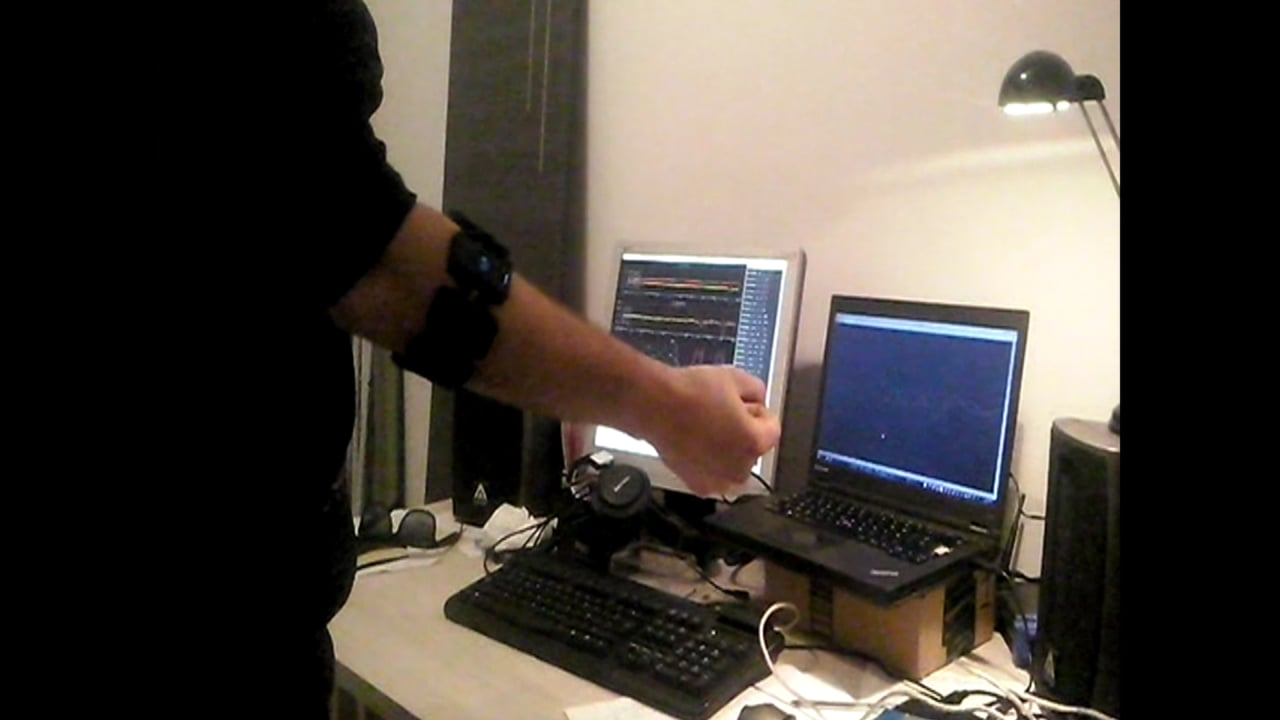
\includegraphics[width=\textwidth]{myosynth.jpg}
    \end{figure}
\end{frame}

\subsection{Multi-level Mappings}

\begin{frame}{Design Considerations - Multi-level Mappings}
    Adding intermediate abstraction layers to the mapping.
\end{frame}

\begin{frame}{Design Considerations - Multi-level Mappings}
    Abstract Layer: 
    \begin{itemize}
        \item Flexibility
        \item Controller/synth mapping independency
    \end{itemize}
\end{frame}

\begin{frame}{Design Considerations - Multi-level Mappings}
    Abstract Layer\blfootnote{Wanderley, M. M., Schnell, N., \& Rovan, J. (1998, October). Escher-modeling and performing composed instruments in real-time.}:
    \begin{figure}[h]
        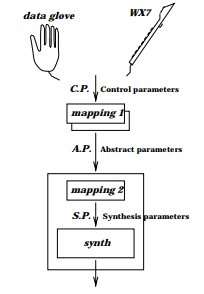
\includegraphics[width=0.35\textwidth]{escher_mapping.png}
    \end{figure}
\end{frame}

\begin{frame}{Design Considerations - Multi-level Mappings}
    2 Abstract Layers: 
    \begin{itemize}
        \item One abstraction for each (controller/synth)
        \item \textit{One-to-one mapping between abstract layers}
    \end{itemize}
\end{frame}

\begin{frame}{Design Considerations - Multi-level Mappings}
    2 Abstract Layers\blfootnote{Based on Hunt, A., Wanderley, M. M., West, S. S., Paradis, M. (2002). The importance of parameter mapping in electronic instrument design, 1–6.}:
    \begin{figure}[h]
        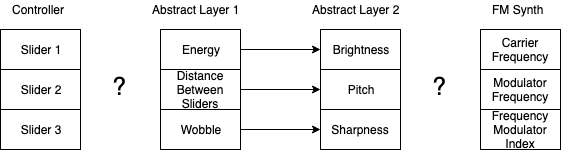
\includegraphics[width=\textwidth]{hunt_2_abstract_layers.png}
    \end{figure}
\end{frame}

\begin{frame}{Design Considerations - Multi-level Mappings}
    \href{https://www.youtube.com/watch?v=0YAOyjPwoJ8}{Reactable SNAP Drum Machine}
    \begin{figure}[h]
        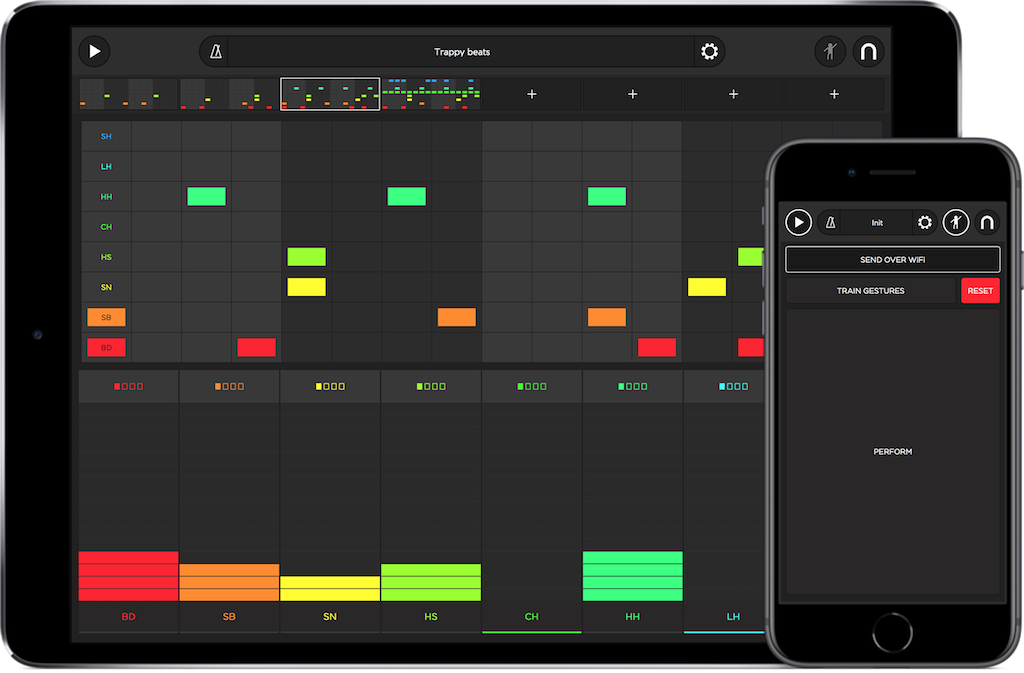
\includegraphics[width=0.8\textwidth]{snap.png}
    \end{figure}
\end{frame}

\subsection{Machine Learning}

\begin{frame}{Design Considerations - Machine Learning}
    \textit{"Machine learning is the scientific study of algorithms and statistical models that computer systems use to effectively perform a specific task \textbf{without using explicit instructions}. [...] Machine learning algorithms build a mathematical model of sample data, in order to make predictions or decisions without being explicitly programmed to perform the task."}\footnote{Wikipedia. Machine Learning. https://en.wikipedia.org/wiki/Machine\_learning. Accessed 17/02/2019}
\end{frame}

\begin{frame}{Design Considerations - Machine Learning}
    Supervised Learning is a great tool for complex/exhausting tasks:
    \begin{itemize}
        \item Classification
        \item Regression
    \end{itemize}
\end{frame}

\begin{frame}{Design Considerations - Machine Learning}
    Classification\blfootnote{proft.me. Types of machine learning algorithms. https://en.proft.me/2015/12/24/types-machine-learning-algorithms. Accessed 17/02/2019.}
    \begin{figure}[h]
        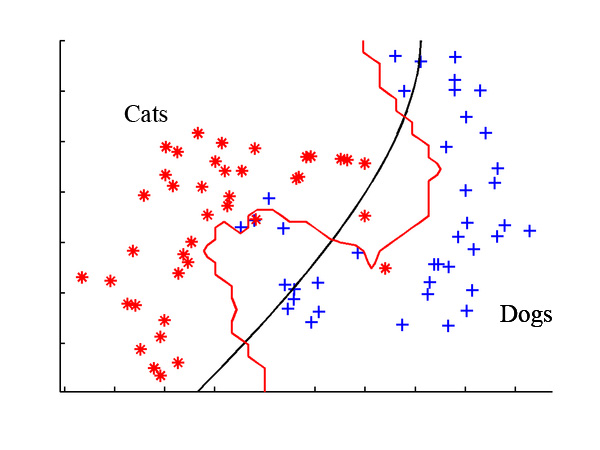
\includegraphics[width=0.65\textwidth]{ml_classification.jpg}
    \end{figure}
\end{frame}

\begin{frame}{Design Considerations - Machine Learning}
    Regression\blfootnote{By Sewaqu - Own work, Public Domain, https://commons.wikimedia.org/w/index.php?curid=11967659}
    \begin{figure}[h]
        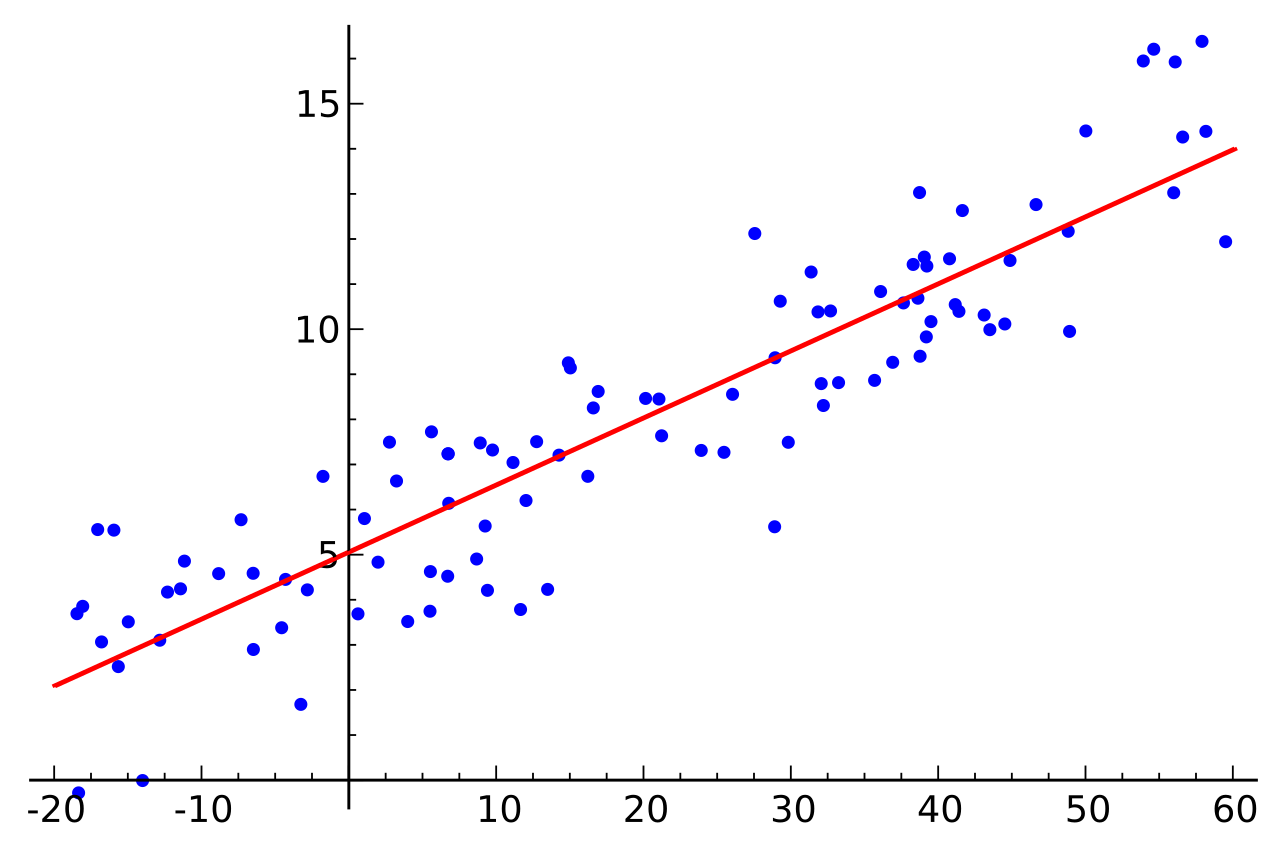
\includegraphics[width=0.75\textwidth]{regression.png}
    \end{figure}
\end{frame}

\begin{frame}{Design Considerations - Machine Learning}
    Supervised Learning: Output types
    \begin{itemize}
        \item Continuous: Regression
        \item Discrete: Classification
    \end{itemize}
    Very interesting for computer-assisted mapping!
\end{frame}

\begin{frame}{Design Considerations - Machine Learning}
    Wekinator\\
    \vspace{5mm}
    \href{https://www.youtube.com/watch?v=dPV-gCqy9j4}{Quick Walkthrough}\\
    \href{https://www.youtube.com/watch?v=NKyyBAKrQgE}{Drum Machine}\\
    \href{ https://www.youtube.com/watch?v=tcQpnV4ajLY}{Face Gesture Recognition}\\
    \href{https://www.youtube.com/watch?v=_mTiXmTGkog}{Non-Linear Mapping}\\
\end{frame}

\end{document}



